\vspace{-0.5em}
\section{Application to Large-Size Decoders}  \label{sec:exp:large}
\vspace{-0.5em}

We also seek to evaluate our method on larger size pre-trained language models (LLMs). 





\subsection{Instruction Tuning and Few-Shot Evaluation} 

LLMs are typically further fine-tuned on curated datasets to tailor them to specific domains and enhance their capacity to follow instructions \citep{wang_23, alpaca, mukherjee_23}. In this section, we employ instruction tuning on these datasets to fine-tune the LLMs and then assess the performance of the resulting models using few-shot benchmarks.

\paragraph{Instruction Tuning.} 
We fine-tune the \mbox{Llama2-7B} model~\citep{touvron_23}
via instruction tuning with the Open-Platypus\footnote{\url{https://huggingface.co/datasets/garage-bAInd/Open-Platypus}}~\citep{lee_23} dataset.
Note that, while Open-Platypus consists of 11 open-source datasets, 
we exclude two of them\footnote{\texttt{leetcode-solutions-python-testgen-gpt4} and \texttt{airoboros-gpt4-1.4.1}} that include outputs from GPT~\cite{DBLP:journals/corr/abs-2303-08774}, and instead use the other nine datasets for fine-tuning. 


\paragraph{Hyper-Parameter Settings.} We conduct all experiments in this section on Nvidia H100 GPU. Following \citet{lee_23}, we fine-tune the model for one epoch, and use a learning rate of $4e^{-4}$ for LoRA~\citep{hu_22} and QLoRA~\citep{dettmers_23}, and $4e^{-5}$ otherwise. We use a batch size of 1 with 32 gradient accumulation steps. We apply the adapters on the feed-forward modules from each layer, following the method described in \citet{he_22}. We prompt the model without step-wise reasoning using the Alpaca~\citep{alpaca} prompt template detailed in \Cref{app:instruct}.



\paragraph{Few-Shot Evaluation.} 
Then, we evaluate our method against other memory-efficient fine-tuning approaches by assessing its performance on several few-shot benchmarks, such as MMLU \citep{hendrycks_21}, ARC easy and challenge \citep{clark_18}, HellaSwag \citep{zellers19}, TruthfulQA \citep{lin_22}, and WinoGrande \citep{DBLP:conf/aaai/SakaguchiBBC20}. We utilize the evaluation scripts provided by the "Language Model Evaluation Harness" \citep{eval-harness}. During the evaluation process, the model outputs the probability associated with closed-form problems defined by the context, question, and multiple potential answers. We select the answer choice with the text associated with the highest probability. 

Table~\ref{tab:llm-perf} reports the accuracy of the model output against the ground truth answer. 
Our method achieves competitive performance gains that are comparable to the performance improvements obtained by other memory efficient fine-tuning approaches. 
We are able to improve the evaluation accuracy upon the base LLama2-7B model, increasing the average accuracy from 60.7 to 61.2. We observe the most significant improvements for TruthfulQA (+3.2) and WinoGrande (+1.0) tasks. We also combine \method with LoRA and QLoRA, further improving the evaluation accuracy compared to the use of \method alone.


	










\begin{table}[t]
 	\centering
\caption{
   Few-shot evaluation results and peak memory usage (GiB) as Llama2-7B is fine-tuned on instruction datasets 
   with (a) \method, (b) \method + LoRA and (c) \method + QLoRA, varying the selection ratio of input tokens. Best results in \textbf{bold}.
 }
 	\label{tab:ablation:tokenratio}
 	\setlength{\tabcolsep}{0.3em}

        \begin{subtable}[c]{0.5\textwidth}
 		\centering
 		\caption{\method{}}
 		\label{tab:ablation:tokenratio:sft}
 		\resizebox{.95\textwidth}{!}{\begin{tabular}{c|c|cccccc}
 			\toprule
 			\makecell[c]{\textbf{Selection}\\\textbf{Ratio}} & \makecell[c]{\textbf{Peak}\\\textbf{Mem.}} & \textbf{MMLU} & \textbf{ARC} & \makecell[c]{\textbf{Hella}\\\textbf{Swag}} & \makecell[c]{\textbf{Truthful}\\\textbf{QA}} & \makecell[c]{\textbf{Wino}\\\textbf{Grande}} & \makecell[c]{\textbf{Avg.}\\\textbf{Perf.}}\\
 			\midrule
 			10\% & \textbf{64.40} & 61.56 & 51.71 & 78.35 & 41.88 & 70.01 & 60.70\\
 			20\% & 65.08 & \textbf{65.01} & 52.65 & \textbf{78.37} & 42.02 & 69.46 & \textbf{61.50}\\
 			30\% & 65.94 & 63.06 & \textbf{53.07} & 77.90 & \textbf{42.18} & 69.93 & 61.23\\
 			40\% & 68.42 & 63.78 & 52.90 & 77.90 & 41.45 & \textbf{70.32} & 61.27\\
 			50\% & 74.32 & 62.98 & 52.73 & 78.32 & 42.11 & 69.38 & 61.10\\
 			\bottomrule
 		\end{tabular}
 		}\end{subtable}
 	
 	\vspace{0.5em}
	
 	\begin{subtable}[c]{0.5\textwidth}
 		\centering
 		\caption{\method{} + LoRA}
 		\label{tab:ablation:tokenratio:lora+sft}
 		\resizebox{.95\textwidth}{!}{\begin{tabular}{c|c|cccccc}
 			\toprule
 			\makecell[c]{\textbf{Selection}\\\textbf{Ratio}} & \makecell[c]{\textbf{Peak}\\\textbf{Mem.}} & \textbf{MMLU} & \textbf{ARC} & \makecell[c]{\textbf{Hella}\\\textbf{Swag}} & \makecell[c]{\textbf{Truthful}\\\textbf{QA}} & \makecell[c]{\textbf{Wino}\\\textbf{Grande}} & \makecell[c]{\textbf{Avg.}\\\textbf{Perf.}}\\
 			\midrule
 			10\% & \textbf{45.47} & 64.17 & \textbf{54.44} & 78.68 & 38.77 & \textbf{69.61} & 61.13\\
 			20\% & 48.21 & 65.41 & 54.35 & \textbf{79.01} & 42.21 & 69.38 & 62.07\\
 			30\% & 52.77 & 65.42 & 54.01 & 78.82 & \textbf{43.78} & 68.35 & 62.08\\
 			40\% & 56.31 & 64.35 & 52.65 & 78.69 & 41.05 & 68.90 & 61.13\\
 			50\% & 64.34 & \textbf{65.87} & 54.01 & 78.68 & 42.46 & 69.38 & \textbf{62.08}\\
 			\bottomrule
 		\end{tabular}
 		}\end{subtable}
 	
 	\vspace{0.5em}
 	
 	\begin{subtable}[c]{0.5\textwidth}
 		\centering
 		\caption{\method{} + QLoRA}
 		\label{tab:ablation:tokenratio:qlora+sft}
 		\resizebox{.95\textwidth}{!}{\begin{tabular}{c|c|cccccc}
			\toprule
			\makecell[c]{\textbf{Selection}\\\textbf{Ratio}} & \makecell[c]{\textbf{Peak}\\\textbf{Mem.}} & \textbf{MMLU} & \textbf{ARC} & \makecell[c]{\textbf{Hella}\\\textbf{Swag}} & \makecell[c]{\textbf{Truthful}\\\textbf{QA}} & \makecell[c]{\textbf{Wino}\\\textbf{Grande}} & \makecell[c]{\textbf{Avg.}\\\textbf{Perf.}}\\
			\midrule
			10\% & \textbf{11.47} & 63.54 & 54.18 & 78.58 & 39.79 & 68.98 & 61.02\\
			20\% & 15.68 & 64.05 & 53.92 & \textbf{78.81} & 40.33 & \textbf{69.85} & 61.39\\
			30\% & 19.71 & \textbf{65.78} & 53.92 & 78.74 & 41.91 & 69.38 & \textbf{61.95}\\
			40\% & 24.11 & 64.85 & \textbf{54.35} & 78.70 & \textbf{41.98} & 69.14 & 61.80\\
			50\% & 31.06 & 65.29 & 53.75 & 78.70 & 40.63 & 69.06 & 61.49\\
			\bottomrule
		\end{tabular}
 		}\end{subtable}
\end{table}


 
%










\subsection{Ratio of Tuned Input Positions}

As done for medium-size encoders in \Cref{sec:medium:ratio}, we then evaluate the impact of the ratio of tuned input positions on the few-shot accuracy. 
We measure the few-shot accuracy of Llama2-7B models fine-tuned using \method with varying ratio of tuned input positions. 
\Cref{tab:ablation:tokenratio} shows few-shot evaluation accuracy of Llama2-7B when the ratio of fine-tuned positions ranges from 10\% to 50\% .


Contrary to what we observed in \Cref{sec:medium:ratio}, we do not necessarily observe a strong correlation between the few-shot accuracy and the ratio of tuned positions. 
In fact, we obtain the best performances most often when 20\%--30\% of input positions are fine-tuned. 
It is important to observe that the average sequence length in these experiments far exceeds the one from the experiments on the GLUE benchmark. This suggests that tuning a relatively small number of positions may be sufficient to successfully fine-tune the model on specific datasets. 

\begin{figure}[t]
\centering
     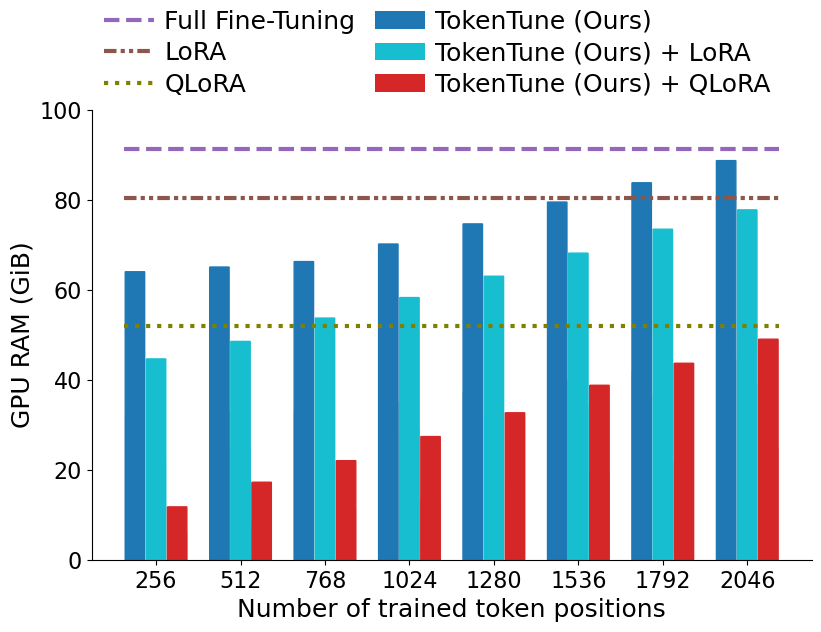
\includegraphics[width=1.0\linewidth]{figures/mem_llama_2.png}
\caption{GPU memory required to fine-tune Llama2-7B~\citep{touvron_23}. We measure the memory by fine-tuning the model on artificially generated data with a given sequence length and batch size. We set the batch size to 1 and the sequence length to \numprint{2048}. We show the memory usage when combining  \method with LoRA and QLoRA and plot the evolution of the memory required to fine-tune the model on a H100 GPU with a number of trained positions ranging between \numprint{256} and \numprint{2046} (we leave at least 2 positions not tuned). 
    Since we could not perform full fine-tuning on our hardware, we estimate the full fine-tuning memory based on the memory reported for \method and LoRA.
    Specific memory usage values can be found in \Cref{tab:gpu_mem_usage}.}
    \label{fig:llm-memory}
\end{figure}

\subsection{GPU Memory Impact}
\label{sec:exp:large:gpu_memory}

As in \Cref{sec:medium:mem}, we analyze the impact of our method on the GPU memory required to fine-tune large language models. \Cref{fig:llm-memory} and \Cref{tab:ablation:tokenratio} report the GPU memory usage for fine-tuning Llama2-7B as the number of trained input tokens changes.
Given an input sequence of length \numprint{2048}, \Cref{fig:llm-memory} shows that our model reduces the memory usage by up to 28\%, from 89 GiB to 64 GiB when reducing the number of trained positions from \numprint{2046} to \numprint{256}. 

The advantage of the proposed method is that it can be combined with other memory saving methods. 
We measure the peak memory required to fine-tune LLama2-7B when combining \method with LoRA or QLoRA. 
Since these approaches target different parts of the memory footprint,
we observe cumulative savings when they are used together. 
When combining LoRA with \method, the peak memory ranges between 78 GiB to 45 GiB depending on the number of tuned positions. 
Similarly, when combining QLoRA with \method, the peak memory decreases from 49 GiB to 12 GiB as a smaller selection ratio is used.

Overall, \Cref{fig:llm-memory} and \Cref{tab:ablation:tokenratio} show that 
the performance of TokenTune is not very sensitive to the choice of token selection ratio, 
while the memory cost is significantly reduced with a smaller token selection ratio.
Based on these results, 
our recommendation is to use 20\%--30\% as the default token selection ratio, and 
test if further improvements in performance and memory usage can be obtained for the given task, with a smaller selection ratio.
